\subsection{\texorpdfstring{DY background estimation in $\tauTau$ channel}{DY background estimation in tau-tau channel}}
The events containing a \Z boson can be an important background in different channels. To evaluate this background, we trust 
the MC, but we validate the MC in a \Z dominated area in data. In the \muTau channel which is defined by the following selections 
\begin{itemize}
\item $\mu$ and \Tau selection similar to signal selection
\item $\mu$ and \Tau are opposite sign (OS)
\item \MPT $>$ 30 
\item b-tag jets are vetoed
\item Extra muon and electron are vetoed 
\item invariant mass of \muTau system $>$ 15 \GeV
\end{itemize}
some selections are modified:
\begin{itemize}
\item \mindphifour cut is removed
\item \mttwo $<$ 20 \GeV
\item 40 $<$\tauMT $<$ 100 \GeV
\end{itemize}
to enrich the \Z events. Figure \ref{fig:ZValidation}(left)
\begin{figure}[h]
\centering
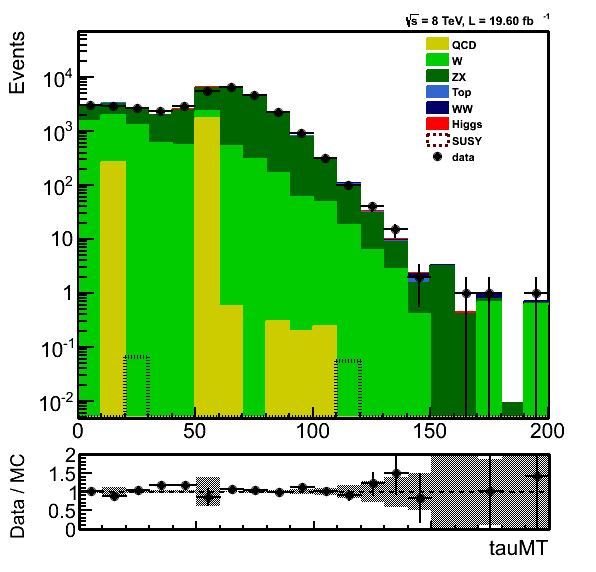
\includegraphics[width=0.475\textwidth,keepaspectratio=true]{ZValidation/tauMT_ZValidation.png}
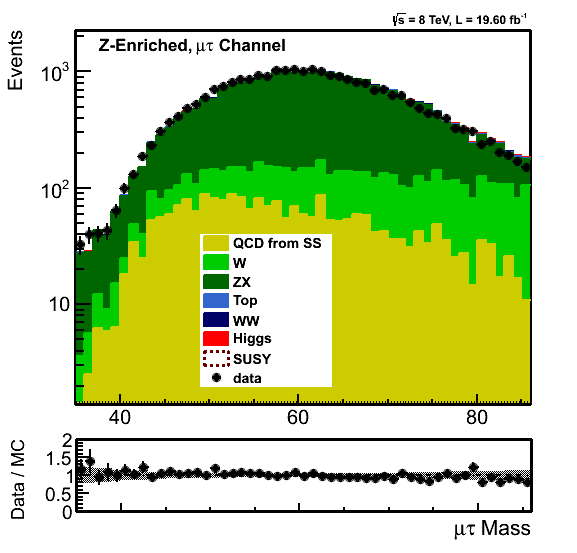
\includegraphics[width=0.475\textwidth,keepaspectratio=true]{ZValidation/InvMass_ZValidation.png}
\caption{left: \tauMT after all other selections to enrich \Z. right: data/MC comparison in the \Z peak.}
\label{fig:ZValidation}
\end{figure}
shows the \tauMT distribution after applying all other selections itemized above. Constraining the \tauMT between 40 and 100 \GeV can increase the \Z contamination from ~70\% to ~80\%. In figure \ref{fig:ZValidation} (right)
dilepton invariant mass is compared between data and MC. The QCD multijet in this plot is estimated from data. For this estimation, the same 
selection is applied as above except the charge of the \muTau which is same (SS) instead of opposite. This condition, enriches the selection 
by QCD multijets (~66\%). The non-QCD backgrounds read from MC are subtracted from data in this selection and the result is 
taken as QCD for the OS selection. All statistical uncertainties on data and MC are considered here, without any extra systematic uncertainty.
It can be seen that data/MC have a good agreement in both shape and normalization under the \Z peak. 

To evaluate the systematics due to 
the extrapolation to the signal region, we look at the \pt of the \Z system in the \Z enriched region.
Figure \ref{fig:ZPtValidation}
\begin{figure}[h]
\centering
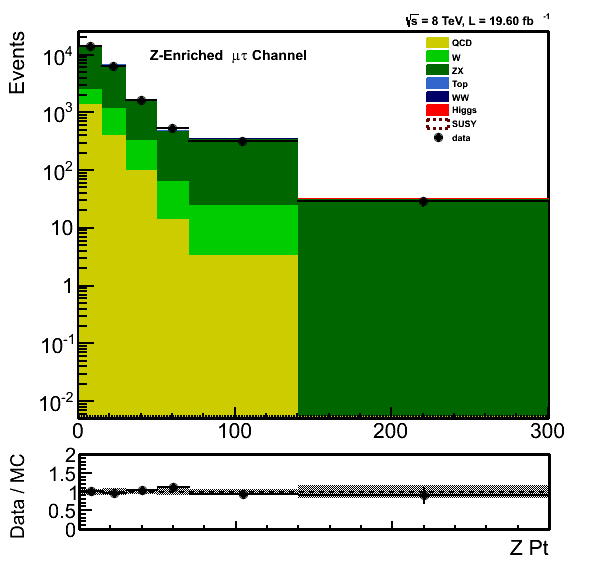
\includegraphics[width=0.45\textwidth,keepaspectratio=true]{ZValidation/ZPt_ZValidation_OSNewQCDSys.png}
\caption{The \pt of the \Z system is used as a probe to look at the signal region. Data/MC agree in the full range within 
  the considered uncertainties.}
\label{fig:ZPtValidation}
\end{figure}
compares data and MC in this region. The QCD is again read from the same sign data when the non-QCD events are subtracted from the data. We have 
considered the statistical uncertainties on data and MC and for all of the MC events in both same sign and opposite sign selections, 25\% 
systematic uncertainties are assigned. It can be seen that the current uncertainties cover the differences between the data and MC in the full 
range of the \pt of the \Z system and no extra systematic is assigned to extrapolate from the control region to the signal region.
Table \ref{Tab.DYbkg}
\begin{table}[!Hhtb]
\begin{center}
\caption{DY background yield expected in four signal regions. The first uncertainty is statistical and the second is systematic. The systematic uncertainties assigned to the central values are discussed in Section \ref{sect:sys}.}
\begin{tabular}{|l|c|}
\hline\hline
Signal Region      &  DY Estimation\\
\hline\hline
\eTau              & 0.20  $\pm$  0.13  $\pm$ 0.05 \\\hline
\muTau             & 0.26  $\pm$  0.13  $\pm$ 0.07 \\\hline
\tauTau \binone    & 0.56  $\pm$  0.07  $\pm$ 0.16 \\\hline
\tauTau \bintwo    & 0.81  $\pm$  0.56  $\pm$ 0.23 \\
\hline\hline
\end{tabular}
\label{Tab.DYbkg}
\end{center}
\end{table}
summarizes the DY contribution in different signal regions. The systematic uncertainties assigned to the central value
are discussed later. For $\ell\Tau$ channels, only the contributions from the prompt lepton + \Tau are reported.
A separate method is developed to estimate the fake contamination in these channels.
